\section{Traffic Management Optimization Using Multi-Objective Evolutionary Algorithms}

Urban traffic management requires balancing multiple conflicting objectives, such as minimizing travel time, reducing fuel consumption, and minimizing air pollution. 
\newline
\newline
In this task, we applied a Multi-Objective Evolutionary Algorithm (MOEA) to optimize traffic management strategies for selected New York City (NYC) areas. The goal is to minimize conflicting 
objectives, Total Travel Time (TTT) and Fuel Consumption (FC), using real-world traffic data from NYC Open Data.
\newline
\newline
The traffic management strategy has involved controlling traffic signal timings (green, yellow, and red light durations), and setting speed limits on these segments. We have developed an MOEA that optimized these parameters to achieve the best trade-off between minimizing TTT and FC.
\newline
\subsection{Data Exploration, and pre processing}
We have used two datasets from the NYC Open Data portal:
1. NYC Traffic Volume Counts[1].
2. Traffic Speed Data[2].
\newline
\newline
The both datasets were collected from New York City Department of Transportation (NYC DOT). The first dataset uses Automated Traffic Recorders (ATR) to collect traffic sample volume counts at bridge crossings and roadways, and contains 31 columns[1], while the second dataset uses average speed of a vehicle traveled between end points, and contains 13 columns[2].
\newline
\newline
\begin{figure}[h]
    \centering
    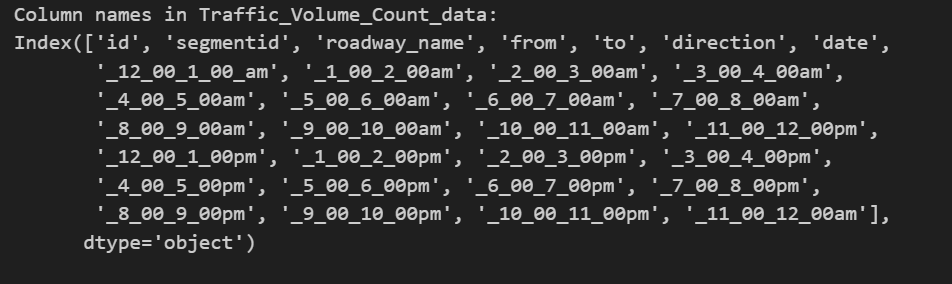
\includegraphics[width=1\linewidth]{figures/trafic_volume_count.PNG}
    \caption{Trafic Volume Count}
    \label{fig:Trafic Volume Count}
\end{figure}
\newline
\begin{figure}[h]
    \centering
    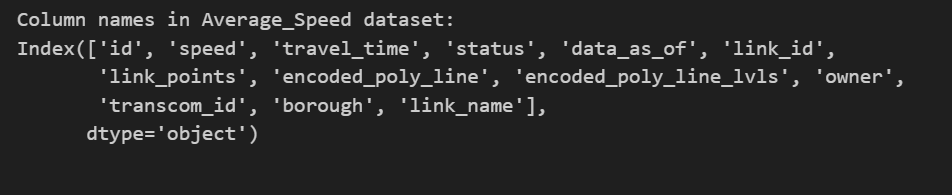
\includegraphics[width=1\linewidth]{figures/average_speed_dataset.PNG}
    \caption{Average Speed Of A Vehicle}
    \label{fig:Average Speed Of a Vehicle}
\end{figure}
\newline
We have focused on optimizing traffic management for the three road segments in New York City, defined as following:
\newline
1. 5th Ave between 46th St and 47th St.
\newline
\begin{figure}[h]
    \centering
    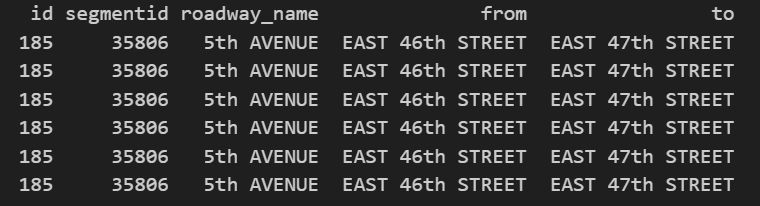
\includegraphics[width=1\linewidth]{figures/area-1.PNG}
    \caption{First 5 columns from First Area}
    \label{fig:Data From Selected Area}
\end{figure}
\newline
2. Atlantic Ave between ALABAMA AVE and WILLIAMS AVE.
\newline
\begin{figure}[h]
    \centering
    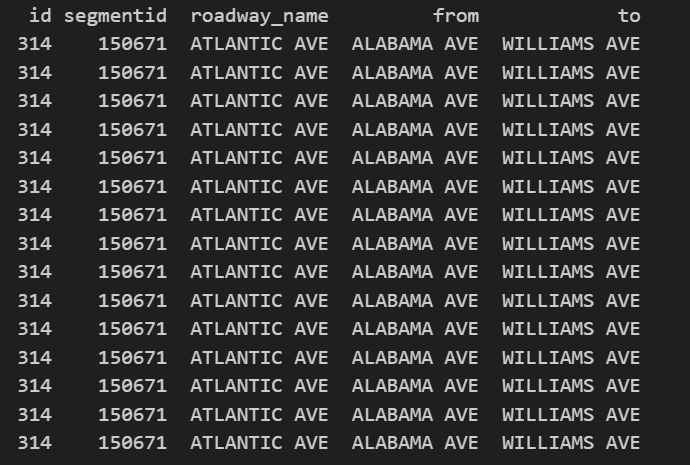
\includegraphics[width=1\linewidth]{figures/area-2.PNG}
    \caption{First 5 columns from Second Area}
    \label{fig:Data From Selected Area}
\end{figure}
\newline
3. Queens Blvd between Union Tpke and Yellowstone Blvd (Queens).
\newline
\begin{figure}[h]
    \centering
    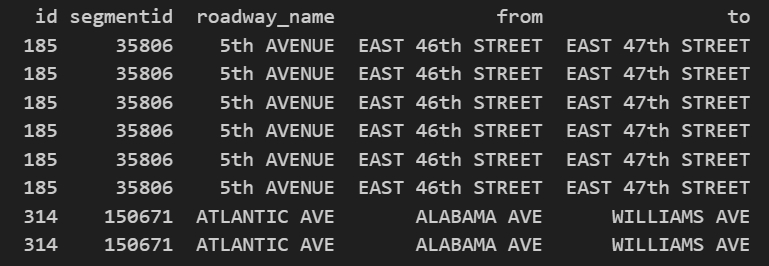
\includegraphics[width=1\linewidth]{figures/area-3.PNG}
    \caption{First 5 columns from Third Area}
    \label{fig:Data From Selected Area}
\end{figure}
\newline
\newline
\begin{figure}[h]
    \centering
    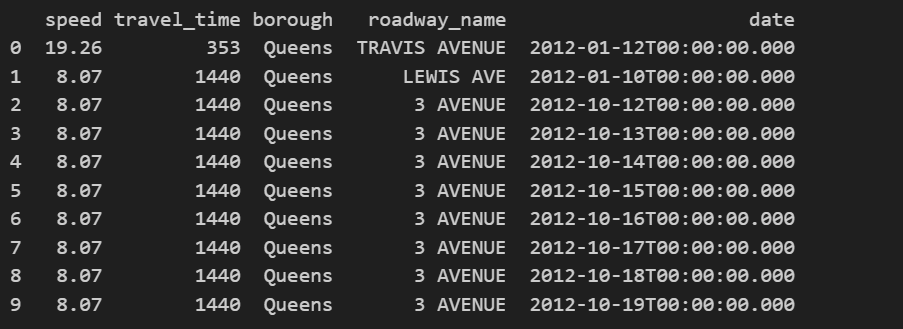
\includegraphics[width=1\linewidth]{figures/data_from_selected_area.PNG}
    \caption{Average Speed Of a Vehicle}
    \label{fig:Data From Selected Area}
\end{figure}
\newline
\newline
In order to use the data from selected area defined above, we have merged all of them in one dataset, which has been merged later with the Trafic Speed Data. Finaly we get one data set named Traffic Volume Count Data For Selected Area. This new dataset contains the sum of the columns of the two original datasets should be 31 + 13 = 44 columns. However, We got an extra column due to the suffixing. 
\newline
\newline
\begin{figure}[h]
    \centering
    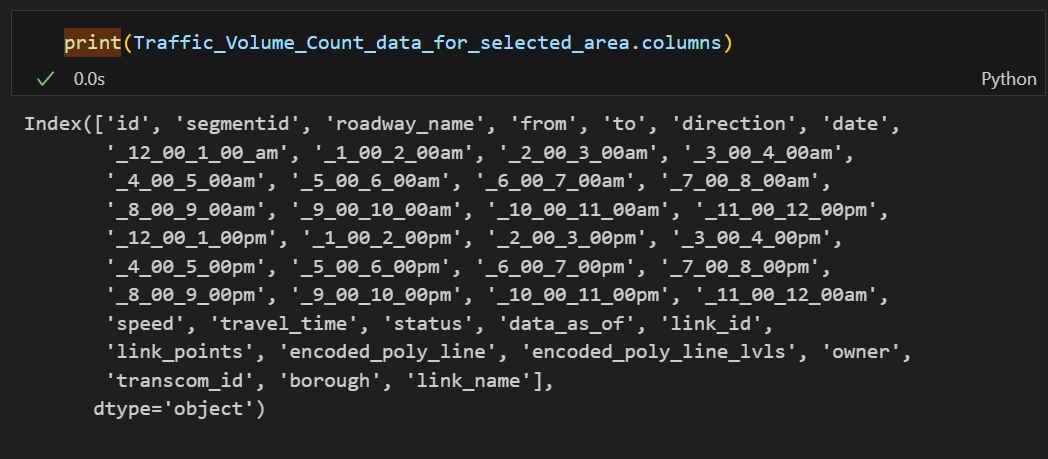
\includegraphics[width=1\linewidth]{figures/mereged_dataset.PNG}
    \caption{Traffic Volume Count Data For Selected Area}
    \label{fig:Traffic Volume Count Data For Selected Area}
\end{figure}
\newline
\newline
We have Identified and preprocess relevant data points, such as:
\newline A. Peak-hour traffic volumes. It has been calculated based on number of travel time in selected hours. In order to achieve this, we have made a list of hourly columns in NewYork City Data. The list defined as following:
\newline
\newline
\begin{figure}[h]
    \centering
    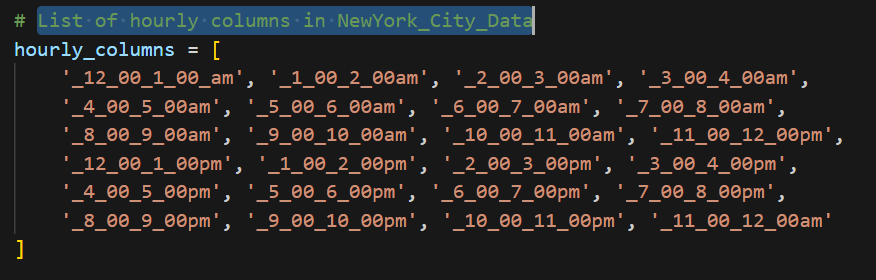
\includegraphics[width=1\linewidth]{figures/List_of_hourly_columns.PNG}
    \caption{Traffic Volume Count Data For Selected Area}
    \label{fig: List Of Hourly Columns in New Yourk City}
\end{figure}
\newline
\newline
To get Overall peak hour, We have identified overall peak hour across all records in dataset, then, we have calculated total traffic for each hour, and got the max volume for each record across the dataset. In the result, the peak hour in New Your City was 7:00 to 8:00 PM, with Overall 8150688 volume.
\newline
\begin{figure}[h]
    \centering
    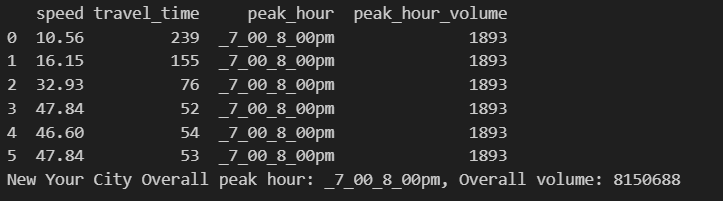
\includegraphics[width=1\linewidth]{figures/peak_huours.PNG}
    \caption{New Your City Peak Huour Time}
    \label{fig:New Your City Peak Huour Time}
\end{figure}
\newline
\newline B. Average speeds.
\newline
In order to calculate the average speed, we have to ensure that the speed data is in numeric type. The mean is a python function allow us to calculate the mean/average of input values or data set. As the result, we found that the average speed is: 2513.80934 mph.
\newline
\subsection{Fuel Consumption Calculation}
Fuel consumption measures the amount of fuel a car consumes to go a specific distance[4]. 
We used the common fuel Consumption equation, defined as following:
\newline
\newline
Fuel Consumption = a × V + b × [1/v] + c
\newline
\newline
Where: 
\newline
\newline
• V is the average speed (in mph). 
\newline
• a, b, and c are empirical const, which a indicating an increase in fuel consumption with speed, while b representing a decrease in fuel consumption as speed, and c represents the base fuel consumption, as very low-speed conditions.
\newline
\newline
However, we sitting a, b, and c values as following:
\newline
Coefficients for the Fuel Consumption Model
\newline a = 0.01  Coefficient for speed (V)
\newline b = 2  Coefficient for 1/V
\newline c = 0.1  Constant term
Then, we have updated the code to calculate Total Fuel Consumption For each road segment, and time interval by defining the formula as following:
\newline
$Fuel Consumption=\sum_{i=1}^{n}  (volume_{i} \times (a×V_{i}+b×\frac{1}{v}+c)\times segment_Length_{i})$
\newline
\newline
where:
\newline n is the number of time intervals. 
\newline Volume is the vehicle count in interval i from the Traffic Volume dataset. 
\newline Vi is the average speed in interval i from the Traffic Speed dataset. 
\newline Segment Length is the length of the road segment.
\newline
\newline
However, from the selected area dataset, 
\newline
peak hourvolume is the vehicle count in the peak hour (Volume).
\newline
\newline speed is the average speed in mph.
\newline segmentid is the Segment length in miles.
\newline
\newline
The following figure shows the data we have used.
\newline
\begin{figure}[h]
    \centering
    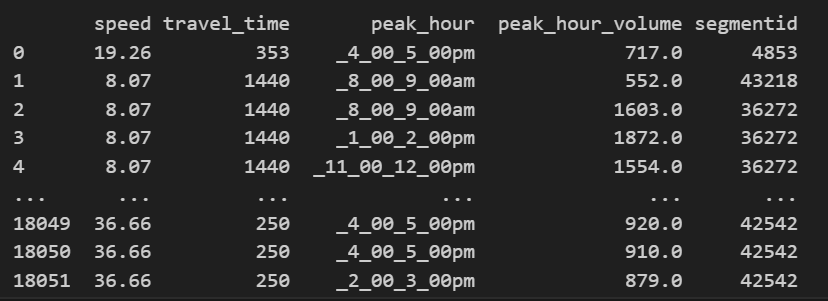
\includegraphics[width=0.7\textwidth]{figures/data_used_to_calculate_Total_Fuel_Consumption_For_each_road_segment.PNG}
    \caption{Selected Area Dataset}
    \label{fig:Selected Area Dataset}
\end{figure}
\newline
The follwoing polt shows the fuel consumption for each time interval.
\newline
\begin{figure}[h]
    \centering
    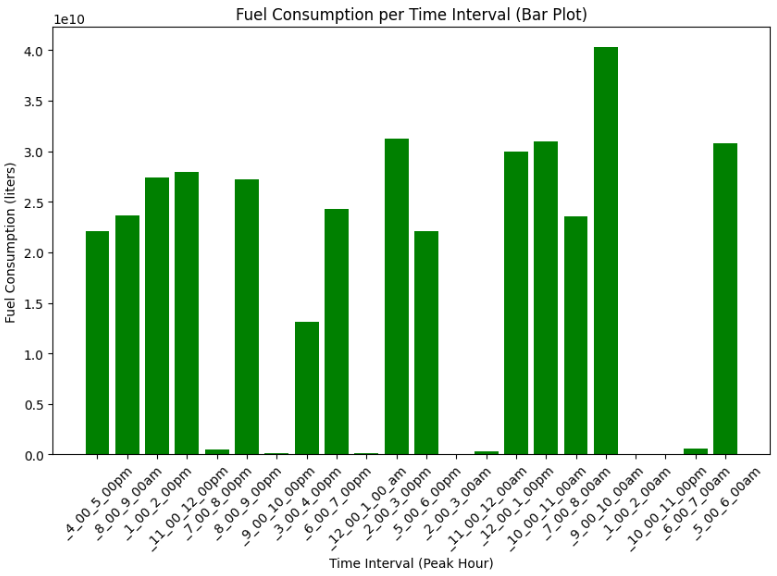
\includegraphics[width=0.7\textwidth]{figures/Fuel_consumption_per_time_interval.PNG}
    \caption{Fuel consumption per time interval}
    \label{fig:Selected Area Dataset}
\end{figure}
\newline
Calculate Total Fuel Consumption:
\newline
$$[\sum_{i=1}^{n}(Volume_{i} \times (a\times V_{i}+b \times \frac{1}{V_{i}}+c) \times segment Length_{i})]$$
\newline
\subsection{Formulate the Optimization Problem}
First, we have defined the Decision Variables: 
\newline A. signaltiming represents the green, yellow, and red signal durations for each intersection.
\newline B. Speed limit













\subsection{Implement the MOEA}
genetic algorithm
\subsection{Analysis and Results}

\begin{figure}[h]
    \centering
    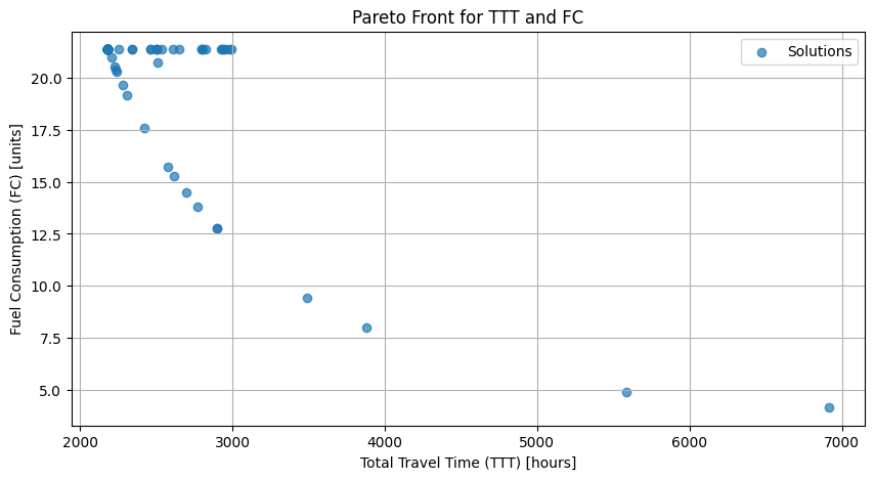
\includegraphics[width=0.7\textwidth]{figures/TTT.PNG}
    \caption{TTT}
    \label{fig:Total Travel Time}
\end{figure}

\begin{figure}[h]
    \centering
    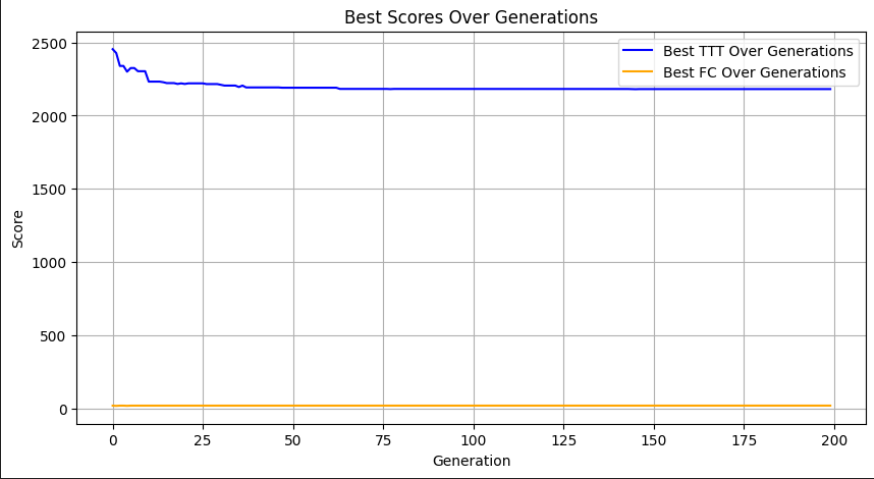
\includegraphics[width=0.7\textwidth]{figures/Best_score.PNG}
    \caption{The best score over generation}
    \label{fig:Best Score Over Generation} 
\end{figure}






